% !TEX root = ../agglo_clust_review.tex
\section{Experiments on CityScapes}\label{sec:cityscapes_exp}
We also evaluate the performances of \algname{} on the CityScapes dataset \cite{cordts2016cityscapes}, which consists of 5000 street-scene images: 2975 for training, 500 for validation and 1525 for testing.
% recorded by car-mounted cameras with resolution 1024$\times$2048: 2975 images for training, 500 for validation and 1525 for testing. Objects with instance-level annotations belong to the following classes: person, rider, car, truck, bus, train, motorcycle, bicycle. 
See Appendix \ref{sec:appendix_cityscapes} for more details on how we fine-tuned the state-of-the-art proposal-free pipeline proposed in GMIS \cite{liu2018affinity} by using a \emph{S\o resen-Dice} loss, similarly to \cite{wolf2018mutex}.
%that achieved superior performances compared to other proposal-based methods like Mark R-CNN and employs a similar model to the one applied by us on neuron-segmentation.
% Their trained model was made publicly available, so we simply replaced their final graph-merging algorithm (MultiStepHAC) with \algname{}.  their instance branch model by using a \emph{S\o resen-Dice} loss similarly to \cite{wolf2018mutex} and obtained in this way sharper affinity-predictions.
Results are summarized in Table \ref{tab:results_cityscapes_val} and Fig. \ref{fig:cityscapes}: similarly to the previous experiments, \algname{} with \emph{Average} linkage achieves the best scores, whereas other linkage tend to over-cluster, like \emph{Abs. Max.}, or under-cluster and merge instances, like \emph{Sum}. The graph-merging algorithm proposed by \cite{liu2018affinity} (MultiStepHAC) requires the user to tune several threshold parameters and it was probably tailored to the original affinities predicted by them, so it did not generalize well to our fine-tuned model and it achieved lower scores compared to the original AP value of 34.1 reported in \cite{liu2018affinity}.  
Appendix - Table \ref{tab:extended_results_cityscapes_val} includes the scores of all other tested \algname{} algorithms.
\begin{figure}[t]
\centering
\begin{minipage}[b]{0.5\textwidth}
    \centering
    \scriptsize
        \begin{tabular}{l|l|cc}
           & Agglomeration  &  \multicolumn{2}{c}{Use constraints:} \\
          Pipeline & method & \textsc{No} & \textsc{Yes} \\ \midrule
DWT \cite{bai2017deep} & - & 21.2 & - \\
SGN \cite{liu2017sgn} & - & 29.2 & - \\
Mask RCNN \cite{he2017mask} & - & 31.5 & - \\ \hline
 & \textbf{\algname{} Avg-Link}& \textbf{34.3}  & 33.9  \\
\multirow{2}{*}{GMIS \cite{liu2018affinity}} & MultiStepHAC \cite{liu2018affinity} & 33.0 & -  \\
 % & \algname{} Max &   24.3  &   32.5  \\
 & \algname{} Abs. Max. \cite{wolf2018mutex}  & 32.1 & 32.1 \\
 & \algname{} Sum \cite{keuper2015efficient,levinkov2017comparative} & 31.3  & 31.9  \\
 % & \algname{} Min &  0    & 0  \\
        \end{tabular}
    \captionof{table}{Average Precision (AP) scores (higher is better) on the CityScapes validation set.}
    \label{tab:results_cityscapes_val}
\end{minipage}\hfill
\begin{minipage}[b]{0.46\textwidth}
    \centering
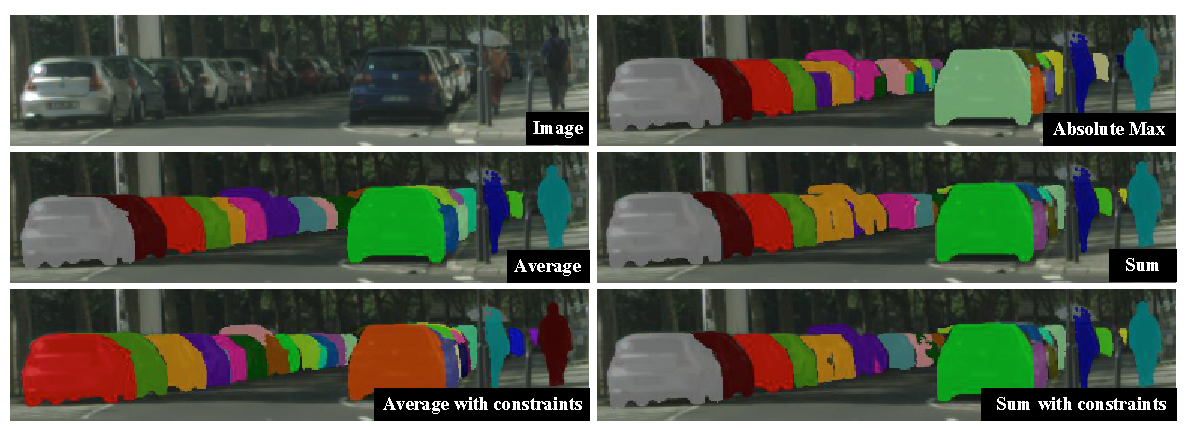
\includegraphics[width=\textwidth]{./figs/cityscapes_compare_3.pdf} % left bottom right top
\caption{Instance segmentations given by different \algname{} linkage criteria on CityScapes}\label{fig:cityscapes}
\end{minipage}
\end{figure}
